\part{Experiments and Critical Assessment}

\chapter{Reading the Experiments}
\label{ch:experiments}

\begin{defbox}[In this chapter you will learn]
\begin{itemize}
 \item how the four shipped demos are configured and what each is designed to show;
 \item how to \emph{interpret} their output with the theory of Parts II and III: a hand-built budget table that predicts who is awake and who collides;
 \item what the numbers actually were (measured, with run-to-run variation);
 \item a worked analysis of the adaptive-ALOHA demo, including a surprising finding about fairness that traces back to the path-loss model;
 \item how to read the paper's Figure~2 and what a faithful reproduction requires.
\end{itemize}
\end{defbox}

\section{The four demos at a glance}
\label{sec:demoglance}

\begin{center}
\footnotesize
\renewcommand{\arraystretch}{1.15}
\begin{tabularx}{\linewidth}{@{}>{\sffamily\bfseries}p{2.3cm}XXXX@{}}
\toprule
 & broadcast & broadcast\_sic & unicast & custom\_protocol\\
\midrule
Question & what do collisions cost? & can SIC remove them? & does polling avoid them? & can a user protocol adapt?\\
Nodes & 3 (2 WPT, 1 hybrid) & 3 & 3 & 12, hybrid\\
Placement & $y=20,30,100$~m north & same & same & random, $r\in[5,40]$~m, seeded\\
BS & 1 mast, 3 sectors, $\SI{46}{dBm}$, $\SI{15}{dBi}$ & same & same & same\\
Beamwidth & $65^\circ$ & $30^\circ$ & $30^\circ$ & $65^\circ$\\
Capacitor & $\SI{300}{\micro F}$ & $\SI{200}{\micro F}$ & $\SI{300}{\micro F}$ & $\SI{300}{\micro F}$\\
Schedule & TX + $2\times$RX$_{10}$ & TX + $3\times$RX$_{15}$ & $3\times$(TX+RX$_{10}$) & policy: TX + $S\times$RX$_8$\\
SIC & off & on & on (default) & on\\
Registration & forced & forced & forced & implicit\\
Horizon & 20 s & 20 s & 20 s & 15 s\\
\bottomrule
\end{tabularx}
\end{center}
All use $\SI{924}{MHz}$, UMa LOS, $\eta=0.7$, node and sector sensitivities of $\SI{-100}{dBm}$, thresholds $1.7/\SI{1.3}{V}$, and the solar trace through a hybrid coverage map for one node (or all, in the custom demo). The first three run in $\approx2$--$4$~seconds of wall-clock time.

\section{A budget table that predicts the results}
\label{sec:budgettable}

Everything the first three demos do follows from five numbers per node, all of which we derived by hand in Parts~II. Collect them:

\begin{center}
\small
\renewcommand{\arraystretch}{1.12}
\begin{tabular}{@{}lrrr@{}}
\toprule
 & Node 0 & Node 1 & Node 2\\
\midrule
Distance north (m) & 20 & 30 & 100\\
UMa LOS path loss (dB) & 60.08 & 62.10 & 71.57\\
Downlink power $P_{\mathrm{dl}}$ (dBm) & $+0.92$ & $-1.10$ & $-10.57$\\
Energy mode & WPT & WPT & hybrid (solar wins)\\
Source voltage $\Vs$ (V) & 2.49 & 1.97 & 2.66 (solar)\\
Time to first $\SI{1.7}{V}$ (s) & 1.8 & 3.4 & 1.6\\
Sustainable current at $\SI{1.5}{V}$ (\si{\micro A}) & 182 & 79 & 218 (solar)\\
Uplink RSSI (dBm) & $-45.7$ & $-49.7$ & $-68.7$\\
\bottomrule
\end{tabular}
\end{center}

\paragraph{Prediction 1: who sends how much?}
Node~1 has the weakest source ($\SI{1.97}{V}$), so it charges slowest and sends least; Node~2 draws on the strong solar source and sends most; Node~0 is in between. The measured packet counts ($20\,\mathrm{s}$, one run): Node~0 $46$, Node~1 $18$, Node~2 $58$. The ordering is exactly that of the sources, \emph{not} that of the distances.

\paragraph{Prediction 2: who loses collisions?}
With SIC off a collision keeps only the \emph{strongest} packet and only if it exceeds the rest by $3$~dB. Node~0 ($-45.7$) is $4.0$~dB above Node~1 ($-49.7$) and $23$~dB above Node~2 ($-68.7$), so it always wins; Node~1 beats Node~2 by $19$~dB; Node~2, the weakest, is the casualty. The measured outcome: decoded $46/46$, $18/18$, $53/58$: \emph{all} errors fall on Node~2.

\paragraph{Prediction 3: SIC removes all errors.}
After capturing Node~0 the remaining pair is $19$~dB apart; SIC recovers it. Measured: $133$ sent, $133$ decoded.

\paragraph{Prediction 4: unicast has no collisions but low answer rate.}
Polling cannot collide; the $20$~s run issued $\approx1333$ polls and decoded $125$ ($\approx9\%$), the rest hitting nodes that were charging.

\section{Measured results}
\label{sec:measured}

Single-run counts vary with the random start-up delays (unseeded). We give the single-run values quoted above together with the ten-seed statistics from our ablation (broadcast scenario, Chapter~\ref{ch:sic}).

\begin{center}
\small
\renewcommand{\arraystretch}{1.12}
\begin{tabular}{@{}lrrrrr@{}}
\toprule
Demo & Sent & Decoded & DER & Throughput & Notes\\
\midrule
broadcast (SIC off) & 122 & 117 & $4.1\%$ & 5.8 pkt/s & errors only on Node~2\\
broadcast\_sic & 133 & 133 & $0.0\%$ & 6.6 pkt/s & \\
unicast & 125 & 125 & $0.0\%$ & 6.2 pkt/s & $\approx9\%$ of polls answered\\
custom\_protocol & 753 & 692 & $8.0\%^\dagger$ & 46.1 pkt/s & 12 nodes, 199 frames\\
\midrule
\emph{10-seed mean, broadcast} & 124.4 & -- & $2.57\%$ ($\pm0.85$) & 6.06 pkt/s & SIC off\\
\emph{10-seed mean, broadcast} & 124.4 & -- & $0.00\%$ & 6.22 pkt/s & SIC on\\
\bottomrule
\end{tabular}
\end{center}
{\footnotesize $^\dagger$ collided share of logged receptions ($60$ of $752$).}

\section{Case study: adaptive framed-slotted ALOHA}
\label{sec:casecustom}

The custom demo runs $12$ hybrid nodes with random placement ($r\in[5,40]$~m, seeded, hence \emph{exactly reproducible}: our run matched the committed CSV to the packet: $753$ sent, $692$ decoded, $60$ collided). The base station starts with $S=20$ slots and adapts (Chapter~\ref{ch:aloha}).

\begin{figure}[t]
\centering
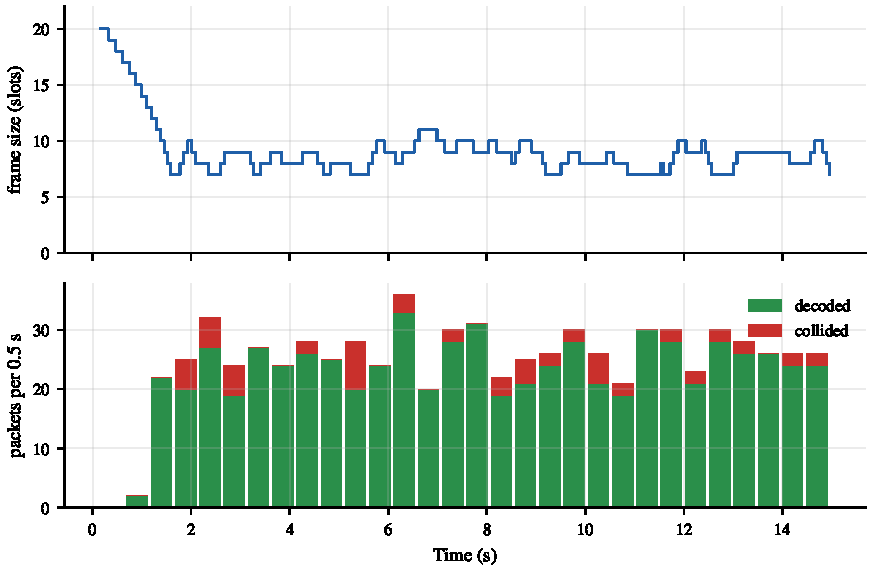
\includegraphics[width=0.82\linewidth]{fig_adaptation}
\caption{Adaptive framed-slotted ALOHA over $\SI{15}{s}$ (from the repository's committed output). Top: frame size per frame; it collapses from $20$ to about $8$ within $\SI{1.5}{s}$ as the BS learns how few nodes are contending. Bottom: decoded and collided packets per $\SI{0.5}{s}$ bin.}
\label{fig:adaptfig}
\end{figure}

\paragraph{Dynamics.} For the first second no node has activated (they are charging), so frames are empty and the policy shrinks the frame by one slot per frame ($20\to7$). From $\SI{0.8}{s}$ nodes start answering; the frame size settles around $S\approx8.4$ with an average of $3.9$ contenders per frame ($3.6$ decoded, $0.3$ collided). Only $\approx4$ of the $12$ nodes contend in any frame: the others are charging, or sit the frame out because of the look-ahead effect of Chapter~\ref{ch:bsengine}.

\paragraph{Collisions are rarer than ALOHA predicts.} With $n=3.9$, $S=8.4$ the textbook probability that a given node's slot is shared is $1-(1-1/S)^{n-1}\approx31\%$. The measured collided share is $8\%$. The difference is due to (i) capture and SIC resolving most pairs (the nodes' powers span $\SI{-66.7}{dBm}$ to $\SI{-14.6}{dBm}$), and (ii) the $5$~ms rule, which lets same-slot packets that start $\ge6$~ms apart coexist.

\paragraph{A surprising fairness result.}
The per-node decoded counts are very uneven:
\begin{center}
\small
\renewcommand{\arraystretch}{1.1}
\begin{tabular}{@{}rrrr|rrrr@{}}
\toprule
node & $r$ (m) & $P_{\mathrm{dl}}$ (mW) & decoded & node & $r$ (m) & $P_{\mathrm{dl}}$ (mW) & decoded\\
\midrule
 3 & 7.0 & 32.6 & \textbf{94} &  0 & 16.3 & 0.63 & 41\\
 4 & 6.3 & 8.2 & \textbf{95} &  1 & 27.8 & 0.11 & 41\\
 5 & 7.4 & 6.1 & \textbf{90} &  2 & 23.8 & 0.33 & 40\\
 7 & 9.3 & 44.3 & \textbf{77} &  6 & 19.9 & 0.63 & 41\\
 \multicolumn{4}{c|}{} & 8,9,10,11 & 25--39 & 0.1--0.8 & 42--44\\
\bottomrule
\end{tabular}
\end{center}
Eight nodes decode an almost identical $40$--$44$ packets, and four decode about twice as many. Both facts follow from the theory.
\begin{enumerate}
 \item The eight ``ordinary'' nodes receive less RF power than the solar trace delivers ($\SI{1.43}{mW}$). With \codew{combine_mode="max"} their energy source is the \emph{same} solar trace, so they have identical energy budgets and, in an uncongested system, identical rates: \emph{energy-limited throughput} (Chapter~\ref{ch:protocols}).
 \item The four ``rich'' nodes lie within $10$~m of the mast, where the RF power ($6$--$\SI{44}{mW}$) \emph{exceeds} the solar power by up to $30\times$, so the max-rule makes RF their source and they recharge much faster.
\end{enumerate}
But $\SI{44}{mW}$ at $\SI{9.3}{m}$ is $+16.5$~dBm, absurdly high for a $\SI{46}{dBm}$ transmitter with a $\SI{25}{m}$ mast: it is the \emph{\textless{}10~m path-loss artefact} of Chapter~\ref{ch:pathloss} (UMa falls through to its second branch and understates the loss by $\sim\SI{14}{dB}$). This is an excellent worked example of how a numerical edge case in the channel propagates, through the energy model, into a protocol-level fairness result. \textbf{The unevenness is not a property of adaptive ALOHA; it is a property of a path-loss branch.} The base station's frame adaptation is working correctly in both cases.

\section{The paper's experiment}
\label{sec:paperexp}

We summarised the experiment and our re-creation in Chapter~\ref{ch:protocols}. Here are practical notes for reading its Figure~2.
\begin{itemize}
 \item The figure is a \emph{box plot}: for each node count, the box spans the interquartile range of the $10$ runs, the centre line (or marker) the median, whiskers the range of non-outliers, dots the outliers. The wide boxes at low density ($\sim80$--$100\%$) reflect the discrete nature of small populations (with $5$ nodes, one failure is $20$ percentage points).
 \item A faithful reproduction needs the \emph{discovery frame parameters}: slot count, slot length, number of rounds, how nodes choose subcarrier shifts, and thresholds/electrical constants; none is given in the abstract. We therefore reproduce \emph{mechanisms}: monotone decay, effect of SIC, role of participation.
 \item With three base stations, a node may be heard by several; the paper's registration counts presumably count a node once. In Amber, ACKs are per base station (each \code{BSBehavior} has its own lists), so you must merge \codew{nodes_registered} across stations.
\end{itemize}

\section{Things to try}

Each is a one-line change that tests a piece of theory.
\begin{enumerate}
 \item \textbf{Capacitance.} Double $C$: the window $\Delta E$ doubles, charge cycles lengthen, packets per cycle rise but the long-run rate (duty-cycle theorem) barely changes.
 \item \textbf{Efficiency $\eta$.} Lower it from $0.7$ to $0.2$: every uplink weakens by $5.4$~dB; the margin of the $\SI{100}{m}$ node over the $\SI{-100}{dBm}$ sector sensitivity shrinks from $31$ to $26$~dB, and its collisions with stronger nodes become harder to resolve.
 \item \textbf{Remove the solar source.} Set \codew{node_energy_mode="wpt"} for all nodes: Node~2 never activates.
 \item \textbf{Move nodes beyond $\SI{10}{m}$} in the custom demo and watch the fairness gap close.
 \item \textbf{Sector power.} Reduce power by $10$~dB; the downlink of Node~1 falls from $-1$ to $\SI{-11}{dBm}$, its $V_\infty$ below $\Vhigh$: it stops.
 \item \textbf{Seeds.} Run any demo ten times and report mean $\pm$ s.d.
\end{enumerate}

\section{Chapter summary}
\begin{itemize}
 \item A five-row budget table (distance, $P_{\mathrm{dl}}$, source voltage, activation time, uplink RSSI) predicts the demos' outcome: who sends how often (by energy source) and who loses collisions (by received power).
 \item The three-node demos are deterministic functions of the budget plus random start-up delays; ten-seed means are the right basis for comparison.
 \item In the adaptive-ALOHA demo only $\sim4$ of $12$ nodes contend per frame; collisions are rarer than textbook ALOHA predicts because of capture, SIC and the $5$~ms rule.
 \item Per-node unevenness in that demo is traced to the $<\SI{10}{m}$ path-loss artefact and the max-rule of hybrid mode, not to the protocol.
\end{itemize}

\section*{Exercises}
\begin{exercise}
Rebuild the budget table for the unicast demo's SIC variant ($30^\circ$ beamwidth). Does the $30^\circ$ beam change any node's gain? (All nodes lie on the boresight.)
\end{exercise}
\begin{exercise}
Using the measured source voltages, estimate the ratio of packets sent by Node~0 and Node~1 from the duty-cycle theorem and compare with $46:18$. Which assumption of the theorem is most violated?
\end{exercise}
\begin{exercise}
In the custom demo, the frame size converges to $\approx8.4$ slots with $\approx3.9$ contenders. Evaluate the slot efficiency of this operating point, and compare it with the $S=n$ and $S=2n$ cases of Section~\ref{sec:energytwist}.
\end{exercise}
\begin{exercise}
Design a ten-seed experiment that isolates the effect of the $<\SI{10}{m}$ artefact on the custom demo's throughput (hint: compare node positions drawn from $[5,40]$ and from $[10,40]$).
\end{exercise}
